\documentclass[12pt]{article}
\usepackage{amssymb, amsmath}
\usepackage{fancyhdr,lastpage}
\usepackage{amsmath,amsfonts,amssymb}
\usepackage{graphicx}
\usepackage{stix}
\usepackage{enumitem}
\usepackage{listings}
\tolerance 10000
\headheight 0in
\headsep 0in
\evensidemargin 0in
\oddsidemargin \evensidemargin
\textwidth 6.5in
\topmargin .25in
\textheight 8.7in

\newcommand{\CC}{{\mathbb C}}
\newcommand{\QQ}{{\mathbb Q}}
\newcommand{\RR}{{\mathbb R}}
\newcommand{\ZZ}{{\mathbb Z}}
\newcommand{\NN}{{\mathbb N}}
\newcommand{\FF}{{\mathbb F}}


\newcommand{\Zerobold}{{\boldsymbol 0}}
\newcommand{\Onebold}{{\boldsymbol 1}}
\newcommand{\xbold}{{\boldsymbol x}}

\newcommand{\mfrak}{{\mathfrak m}}

\newcommand{\Acal}{{\mathcal A}}
\newcommand{\Ncal}{{\mathcal N}}
\newcommand{\Pcal}{{\mathcal P}}
\newcommand{\Qcal}{{\mathcal Q}}

\newcommand{\sqbinom}[2]{\genfrac{[}{]}{0pt}{}{#1}{#2}}
\newcommand{\angbinom}[2]{\genfrac{\langle}{\rangle}{0pt}{}{#1}{#2}}

\newcommand{\qddx}{(d/dx)_{q}}

%\newcommand{\pfcl}{\emph{Proof of claim}}
\newenvironment{proof}{\paragraph{Proof: }}{\hfill$\blacksquare$}



\def\multiset#1#2{\ensuremath{\left(\kern-.3em\left(\genfrac{}{}{0pt}{}{#1}{#2}\right)\kern-.3em\right)}}


\DeclareMathOperator{\des}{des}
\DeclareMathOperator{\maj}{maj}
\DeclareMathOperator{\ev}{ev}
\DeclareMathOperator{\Hom}{Hom}
\DeclareMathOperator{\trace}{tr}
\DeclareMathOperator{\inv}{inv}

\newtheorem{problem}{Problem}%[section]

\begin{document}

\begin{center}
{\bf Julio Soldevilla}
\\
{\bf EECS 545 Winter 2018 --- Problem Set 5 }
\end{center}

\begin{problem}
\normalfont
Problem 1
\end{problem}

\begin{proof}

\begin{figure}[!htbp]
\centering
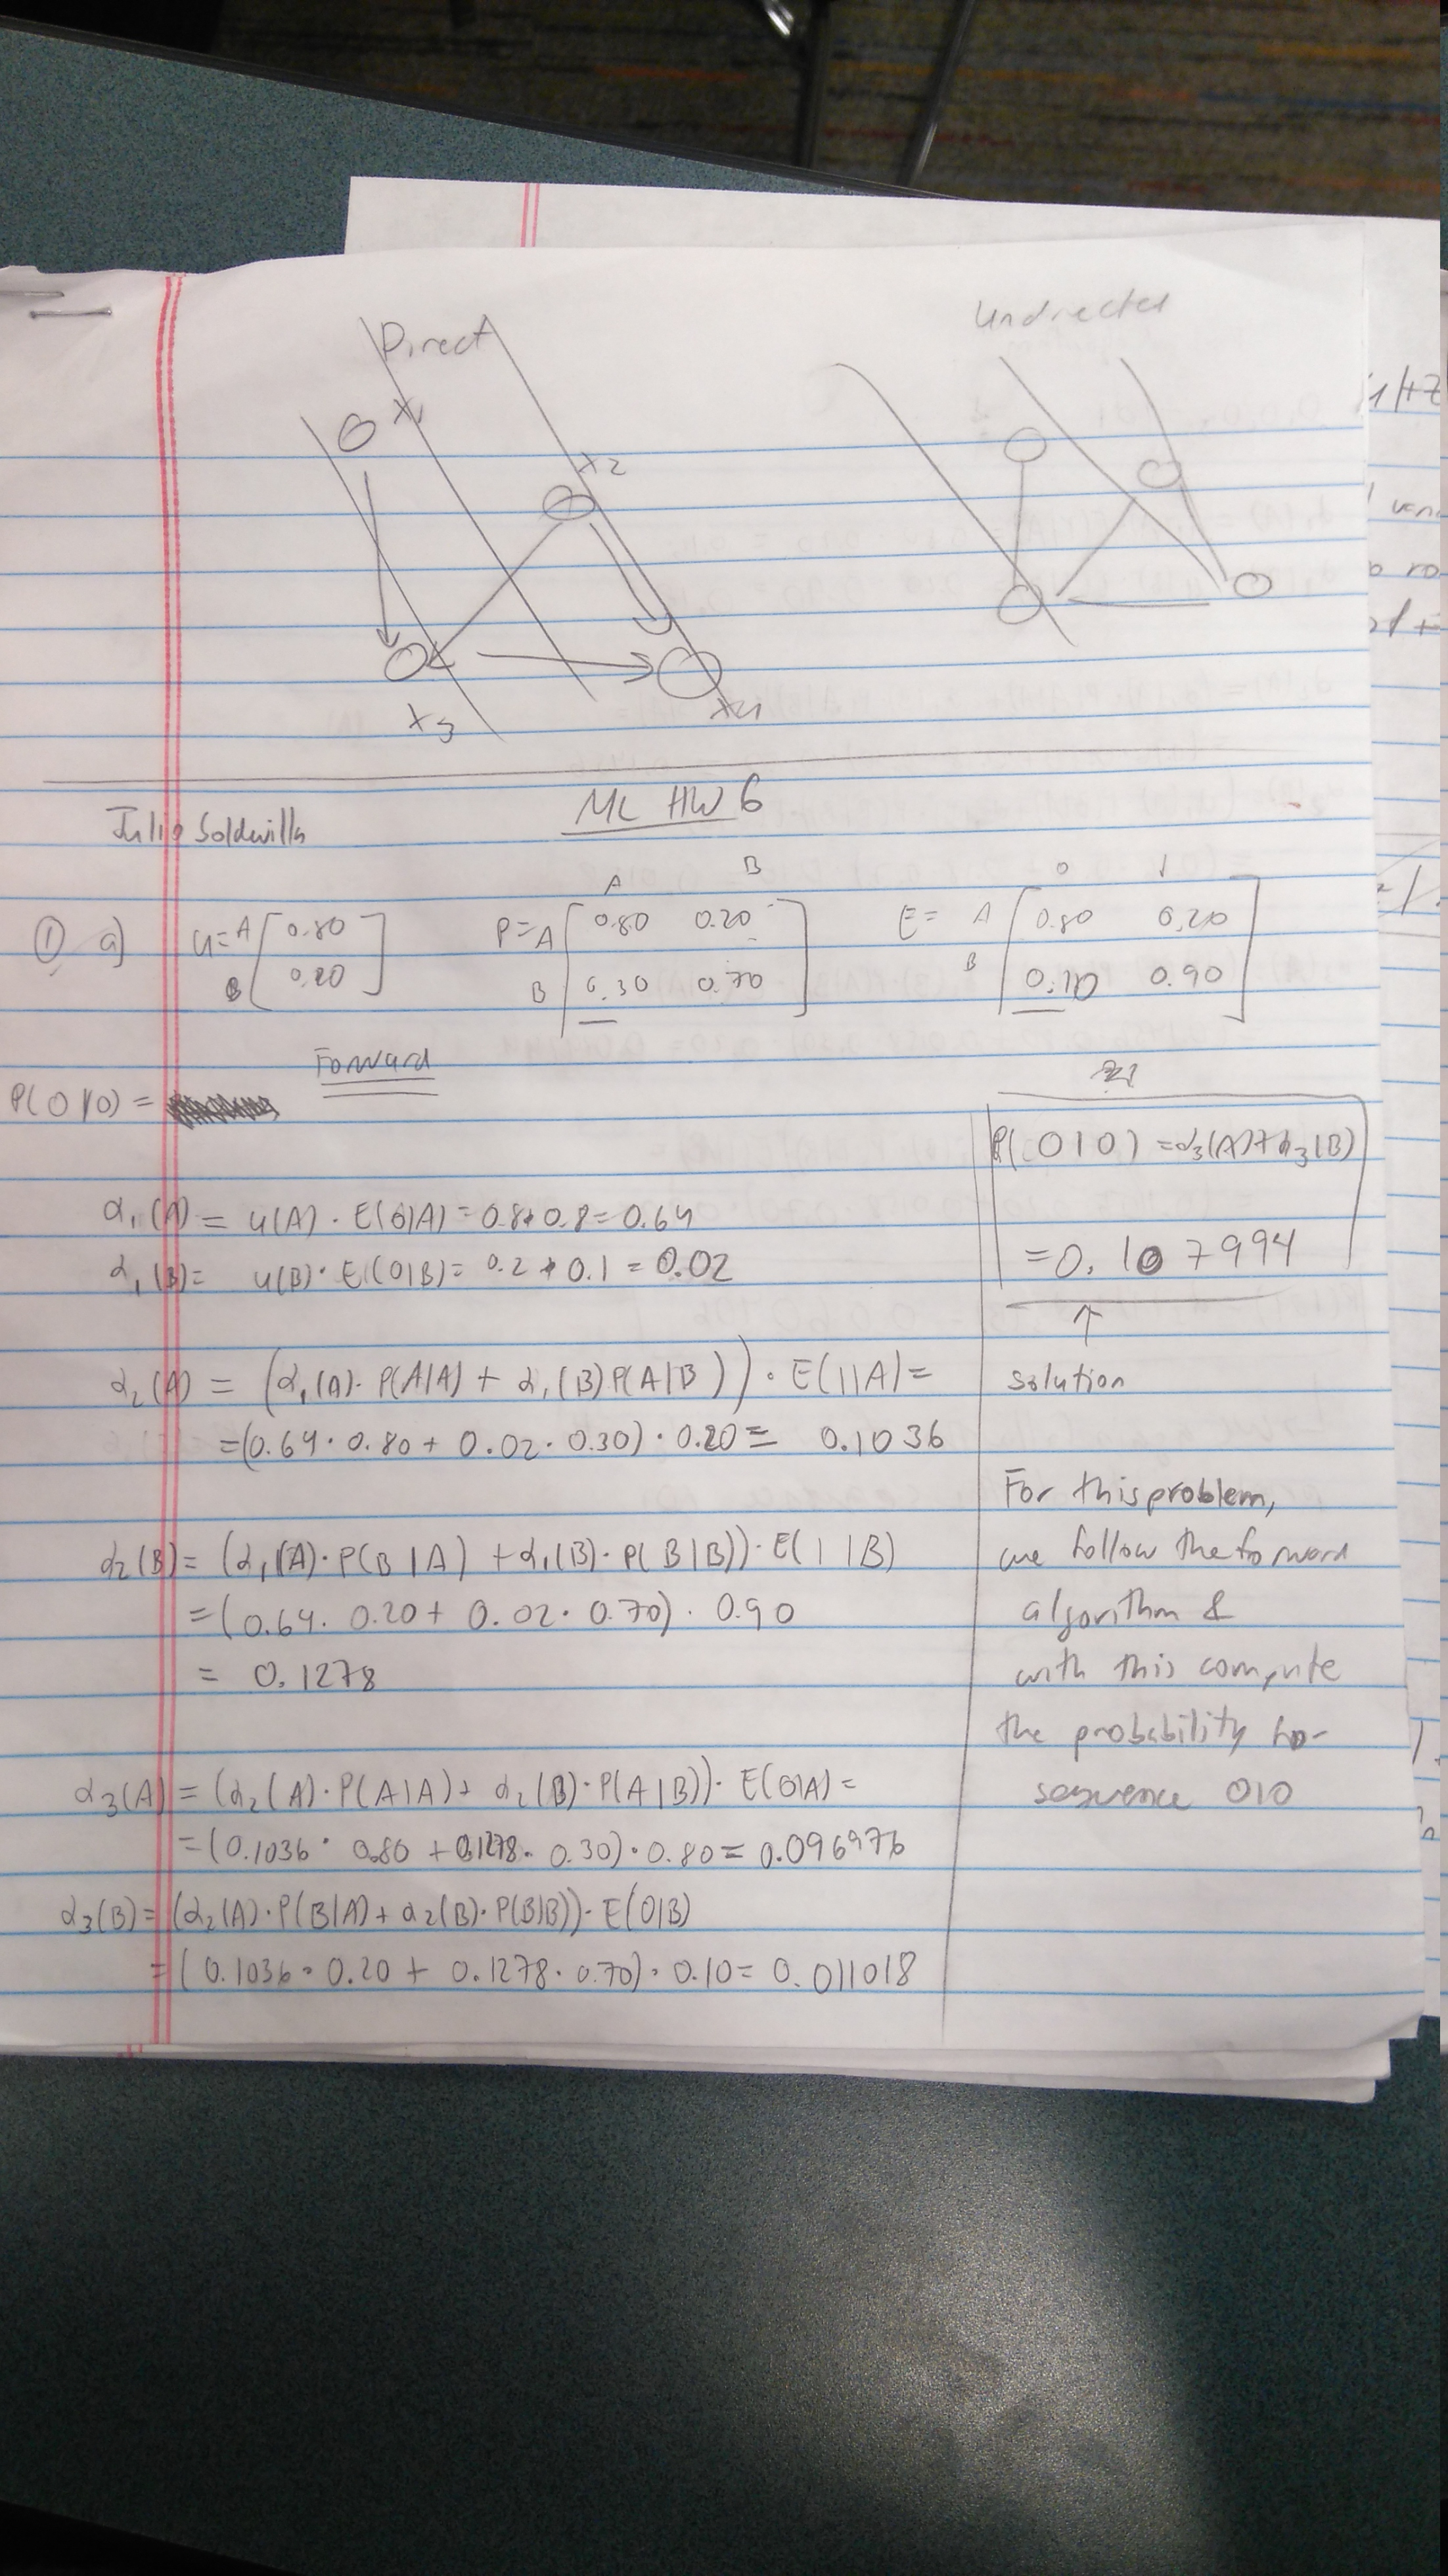
\includegraphics[width = 13cm]{hw6_1a_1.jpg}
\caption{\textbf{Problem 1 part a :} Image showing the work for 1 sequence 010}
\end{figure}
\newpage

\begin{figure}[!htbp]
\centering
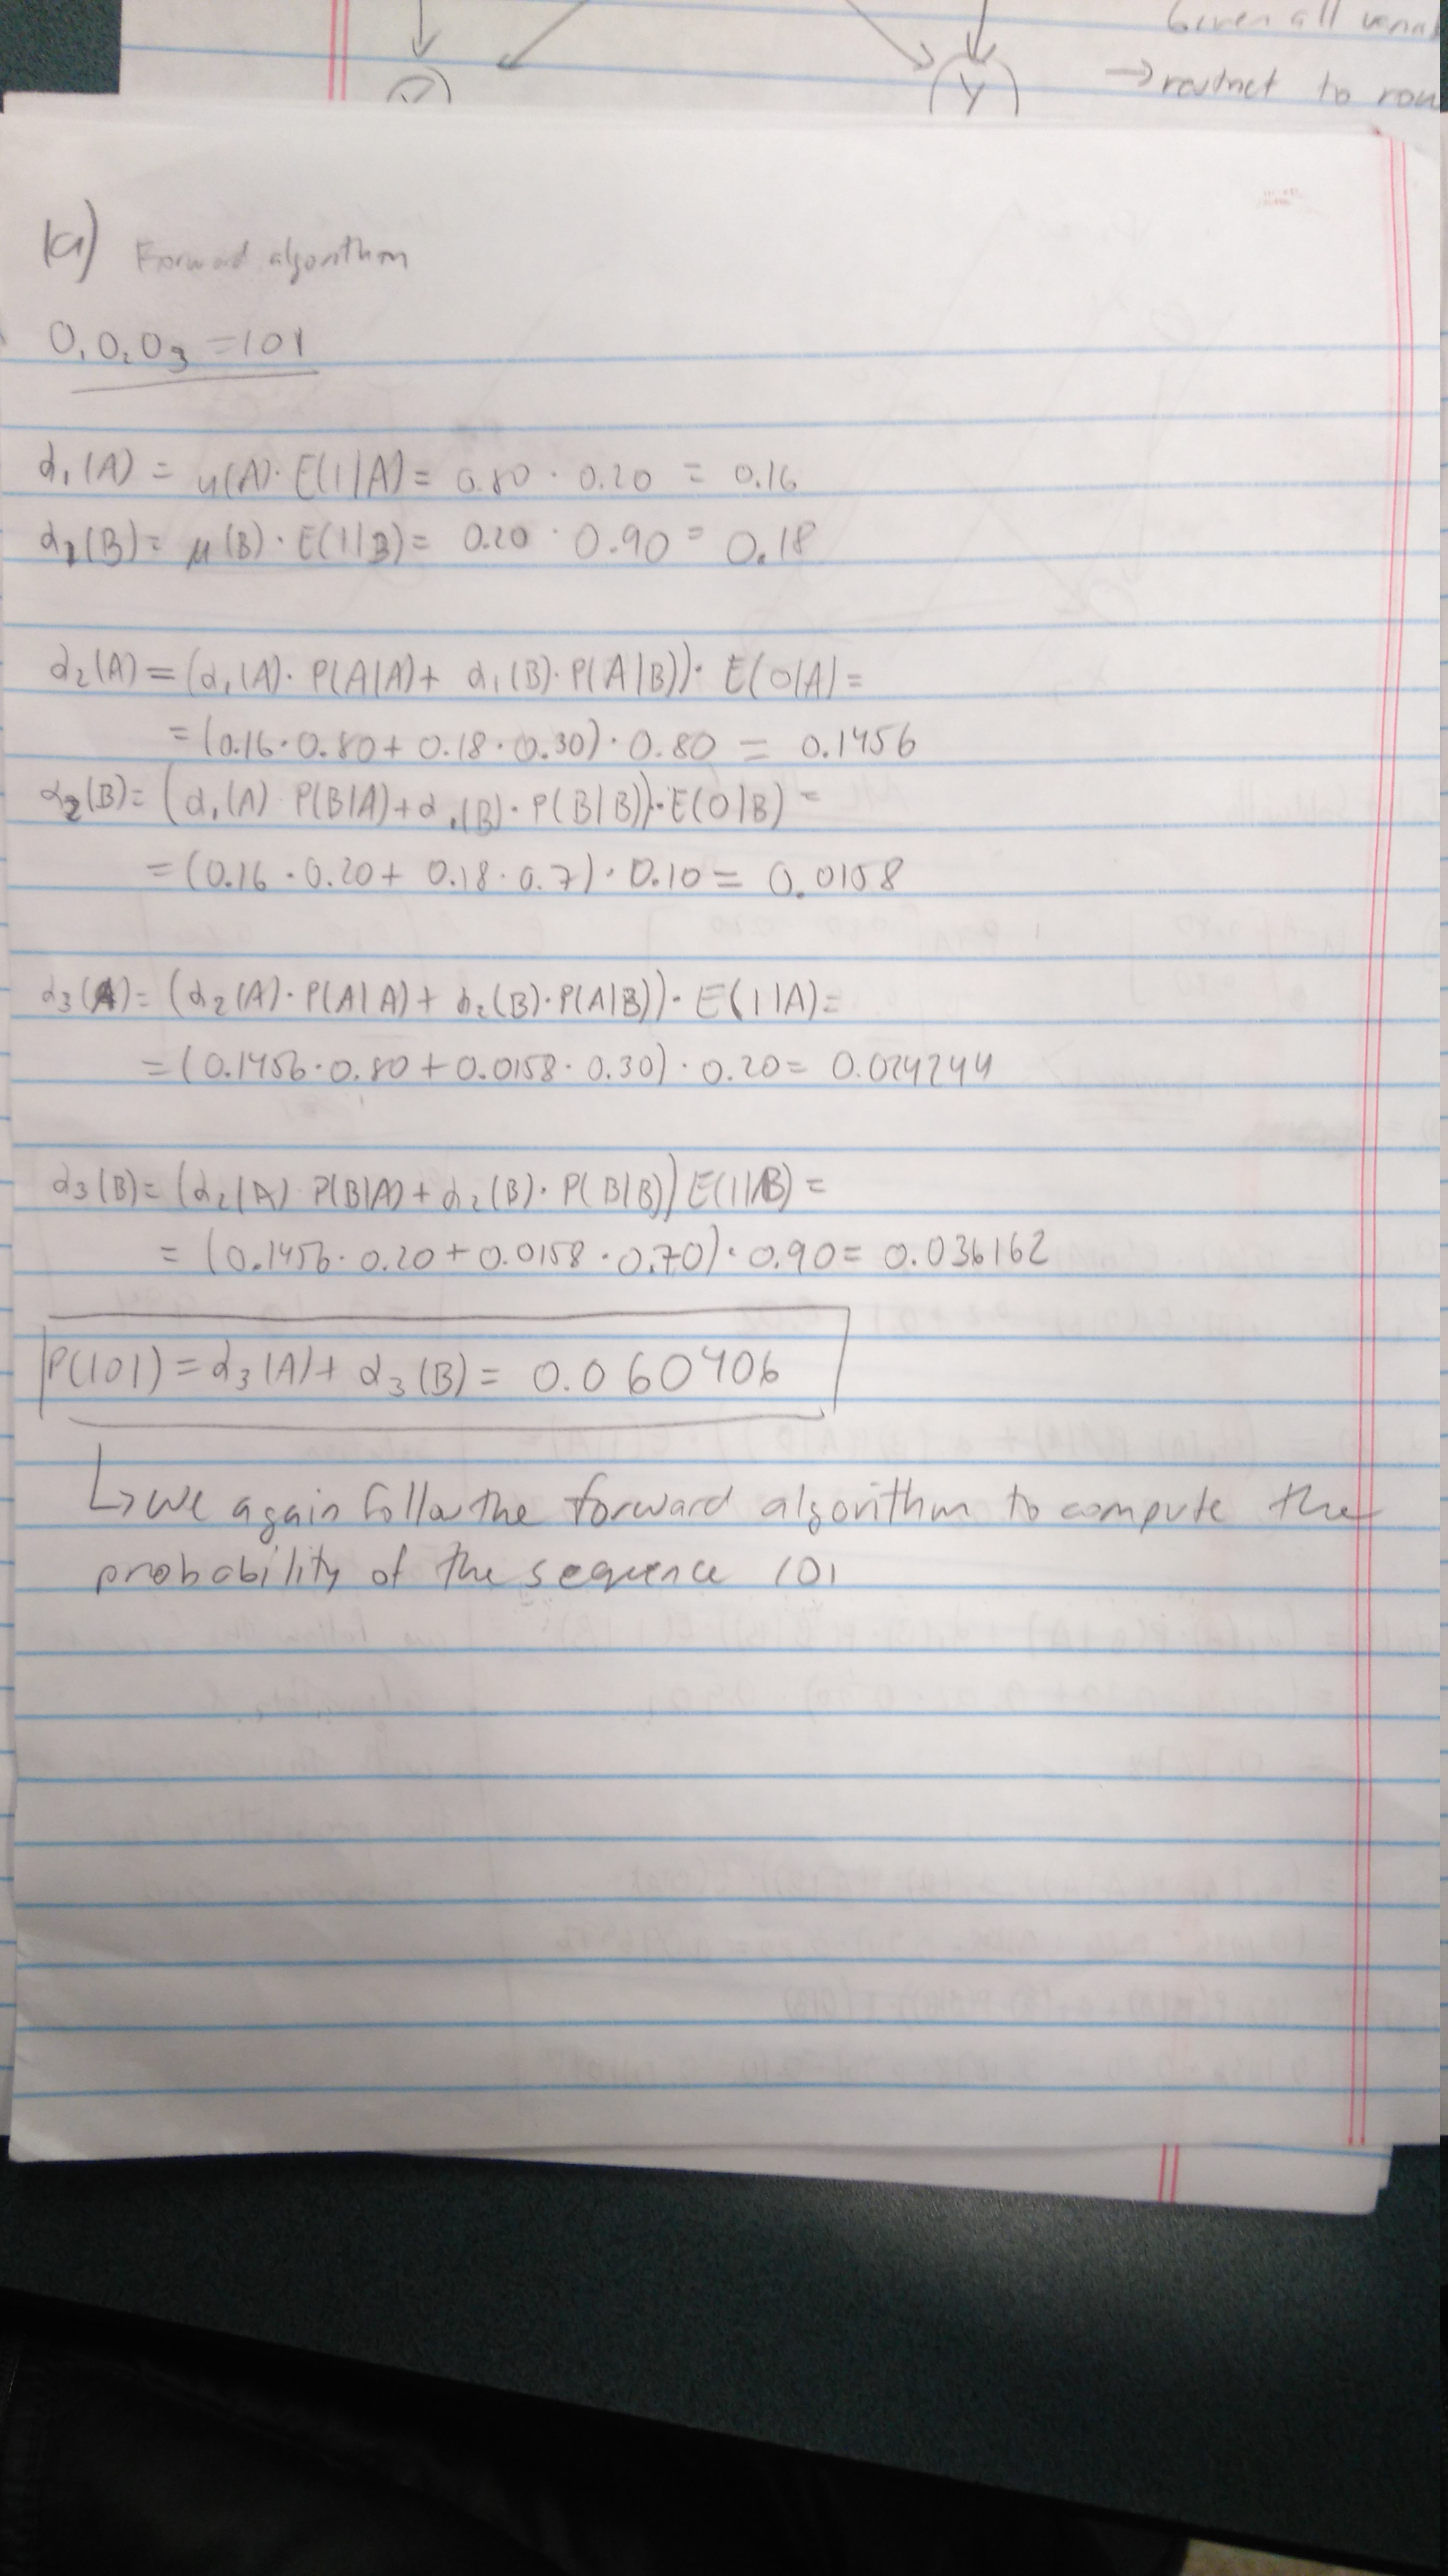
\includegraphics[width = 13cm]{hw6_1a_2.jpg}
\caption{\textbf{Problem 1 part a :} Image showing the work for 1 sequence 101}
\end{figure}

\newpage

\begin{figure}[!htbp]
\centering
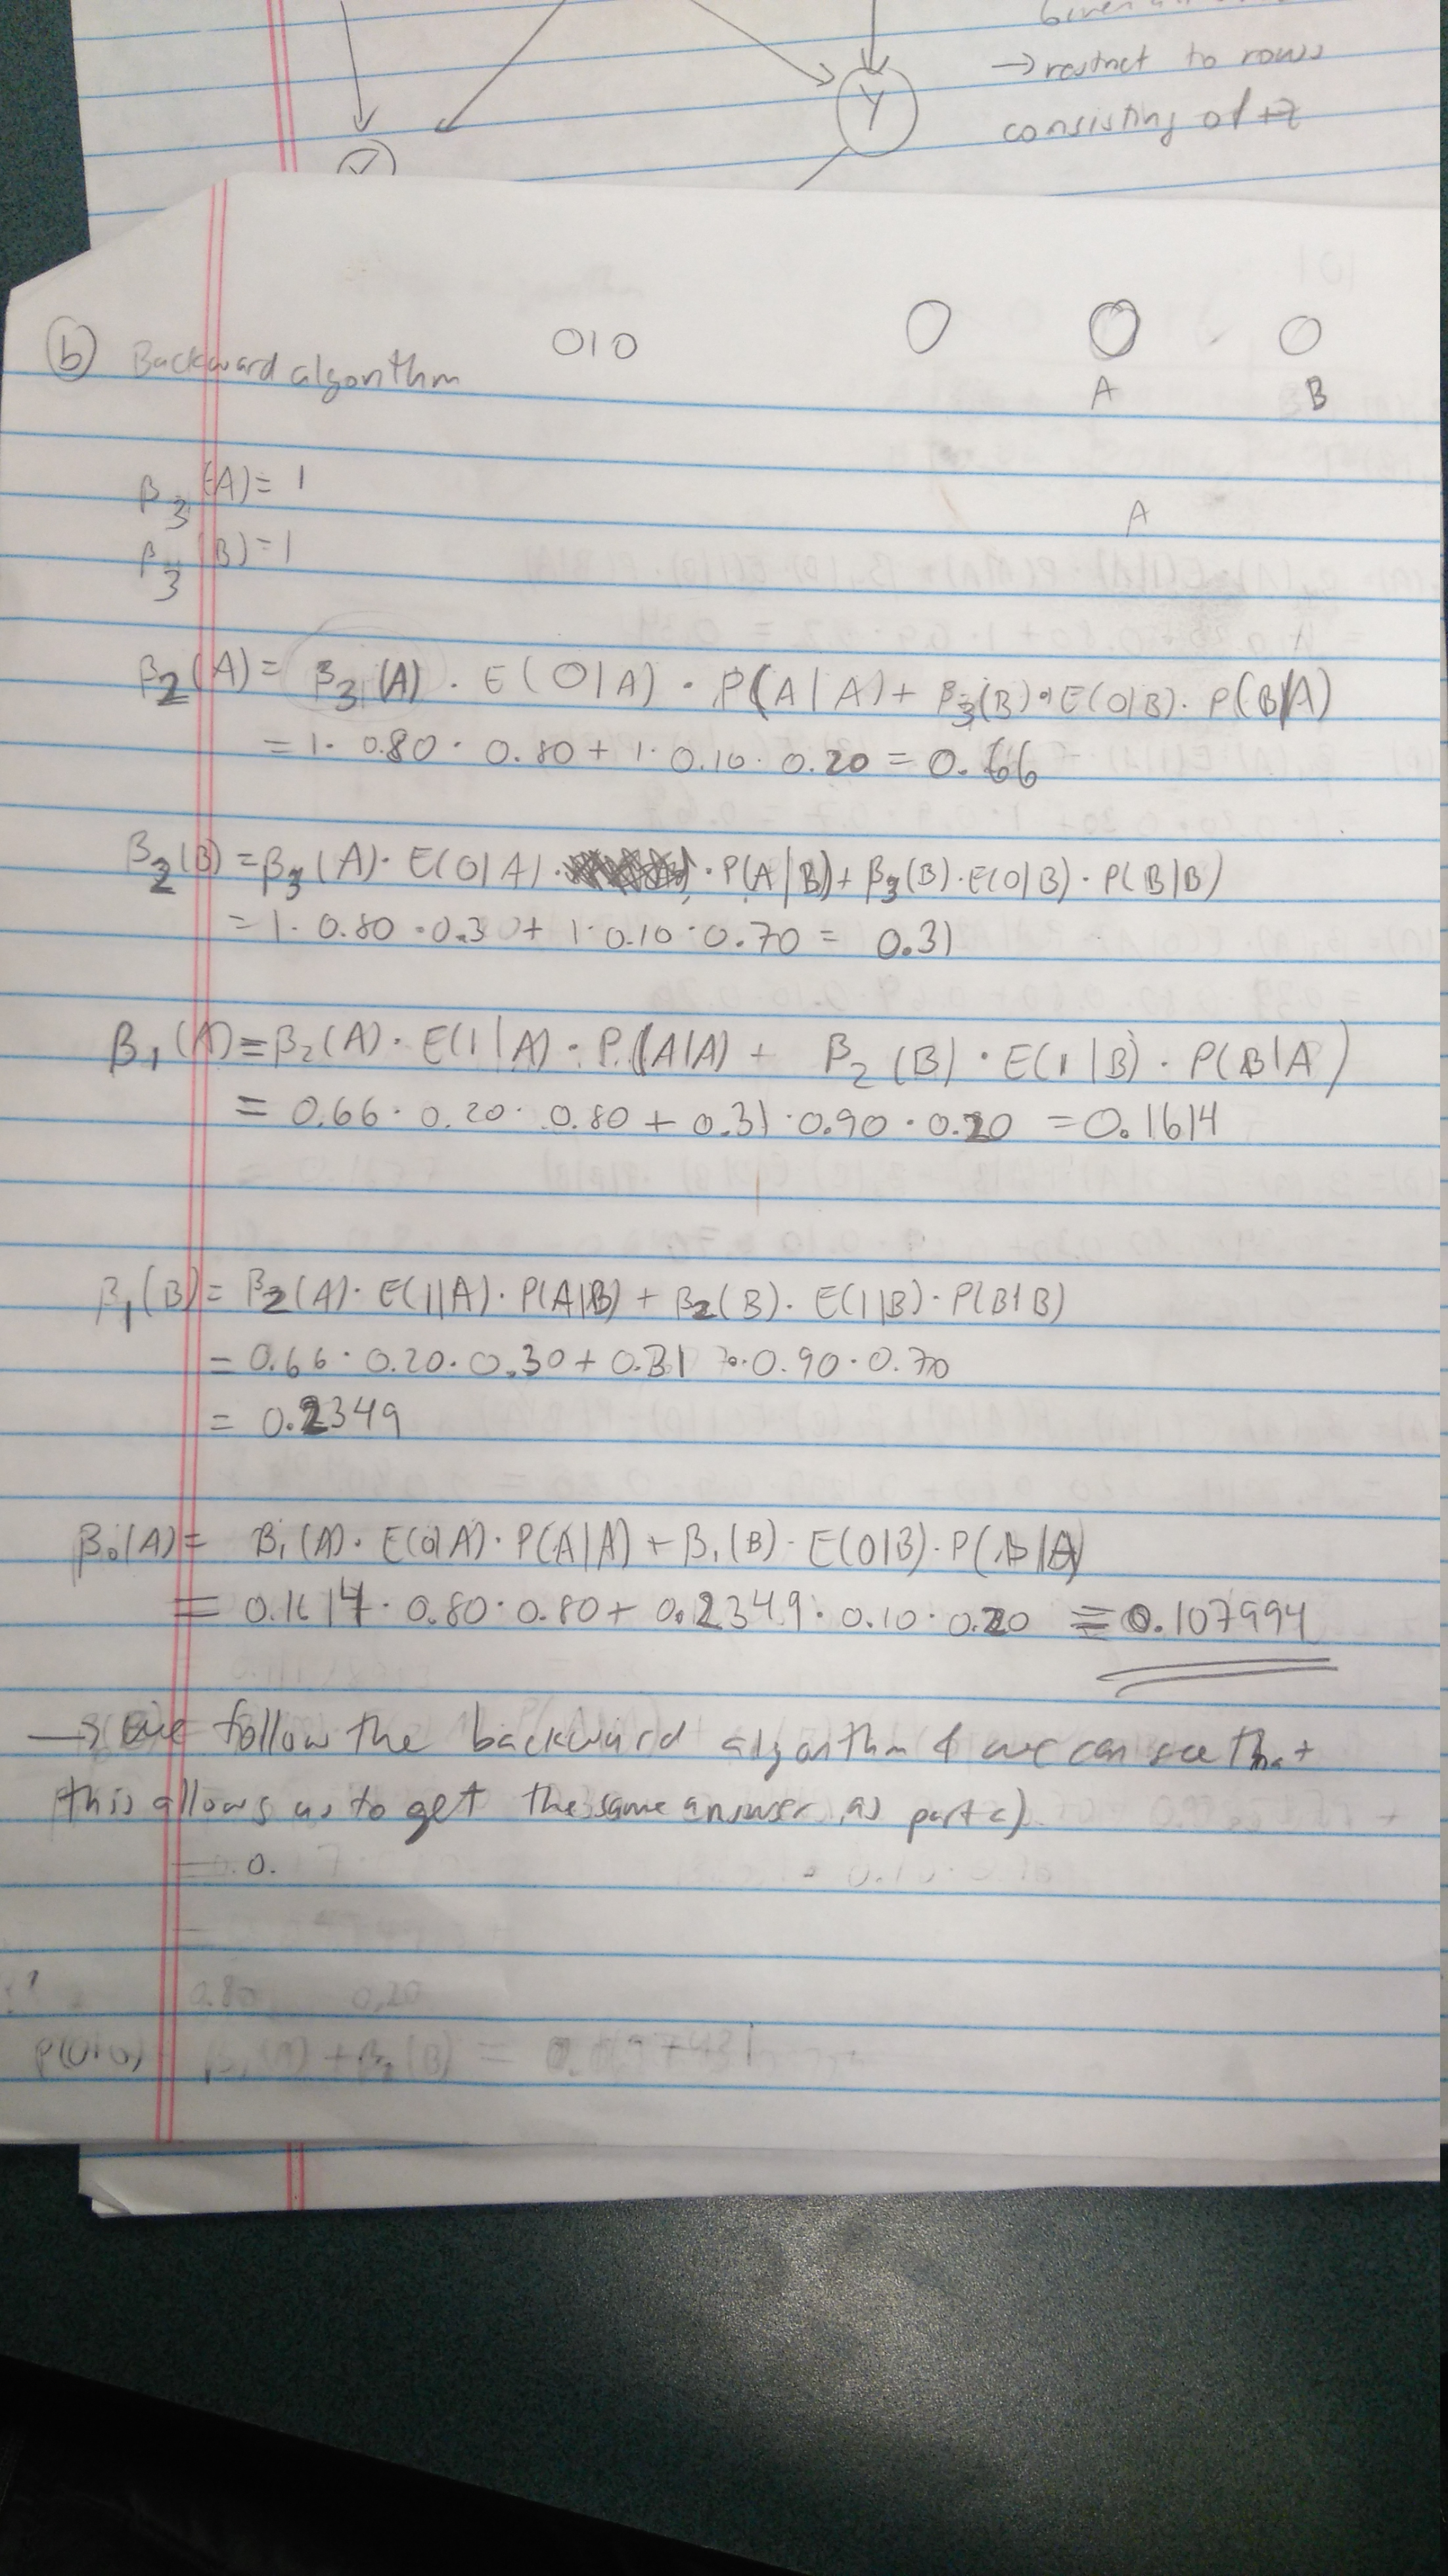
\includegraphics[width = 13cm]{hw6_1b_1.jpg}
\caption{\textbf{Problem 1 part b:} Image showing the work for 1 sequence 010 backward alg}
\end{figure}

\newpage
\begin{figure}[!htbp]
\centering
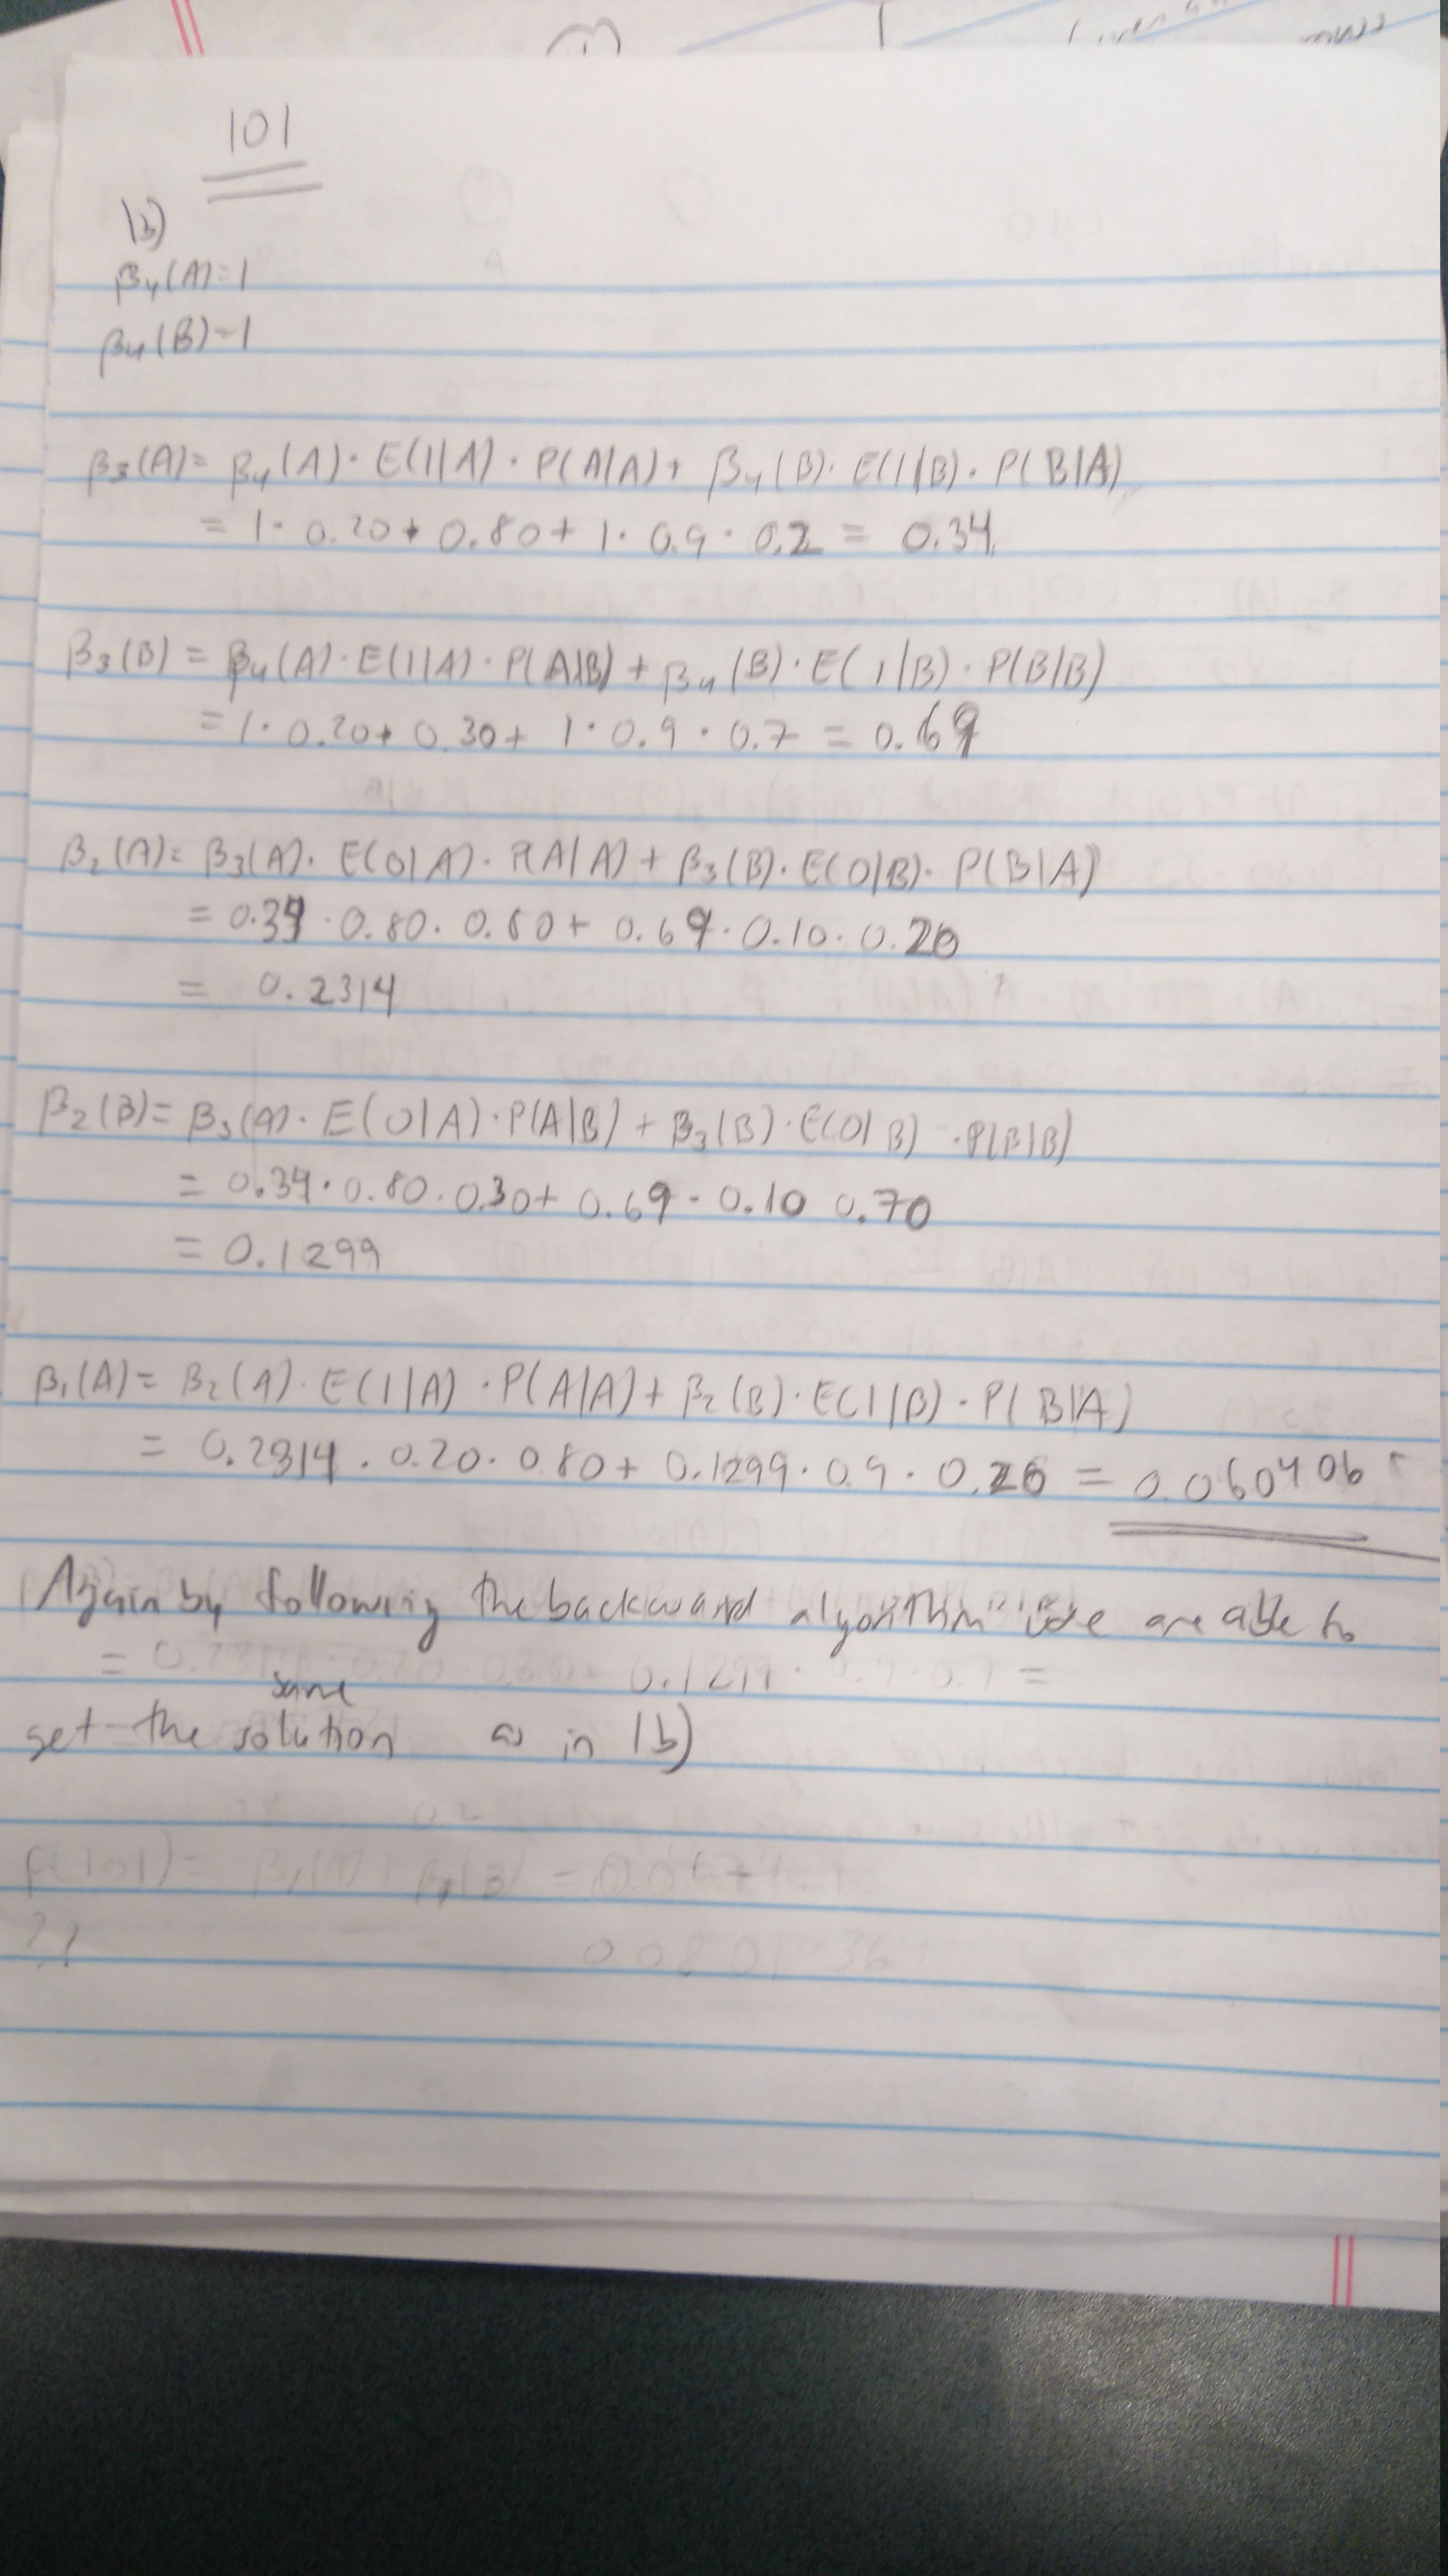
\includegraphics[width = 13cm]{hw6_1b_2.jpg}
\caption{\textbf{Problem 1 part b:} Image showing the work for 1 sequence 101 backward alg}
\end{figure}

\newpage

\begin{figure}[!htbp]
\centering
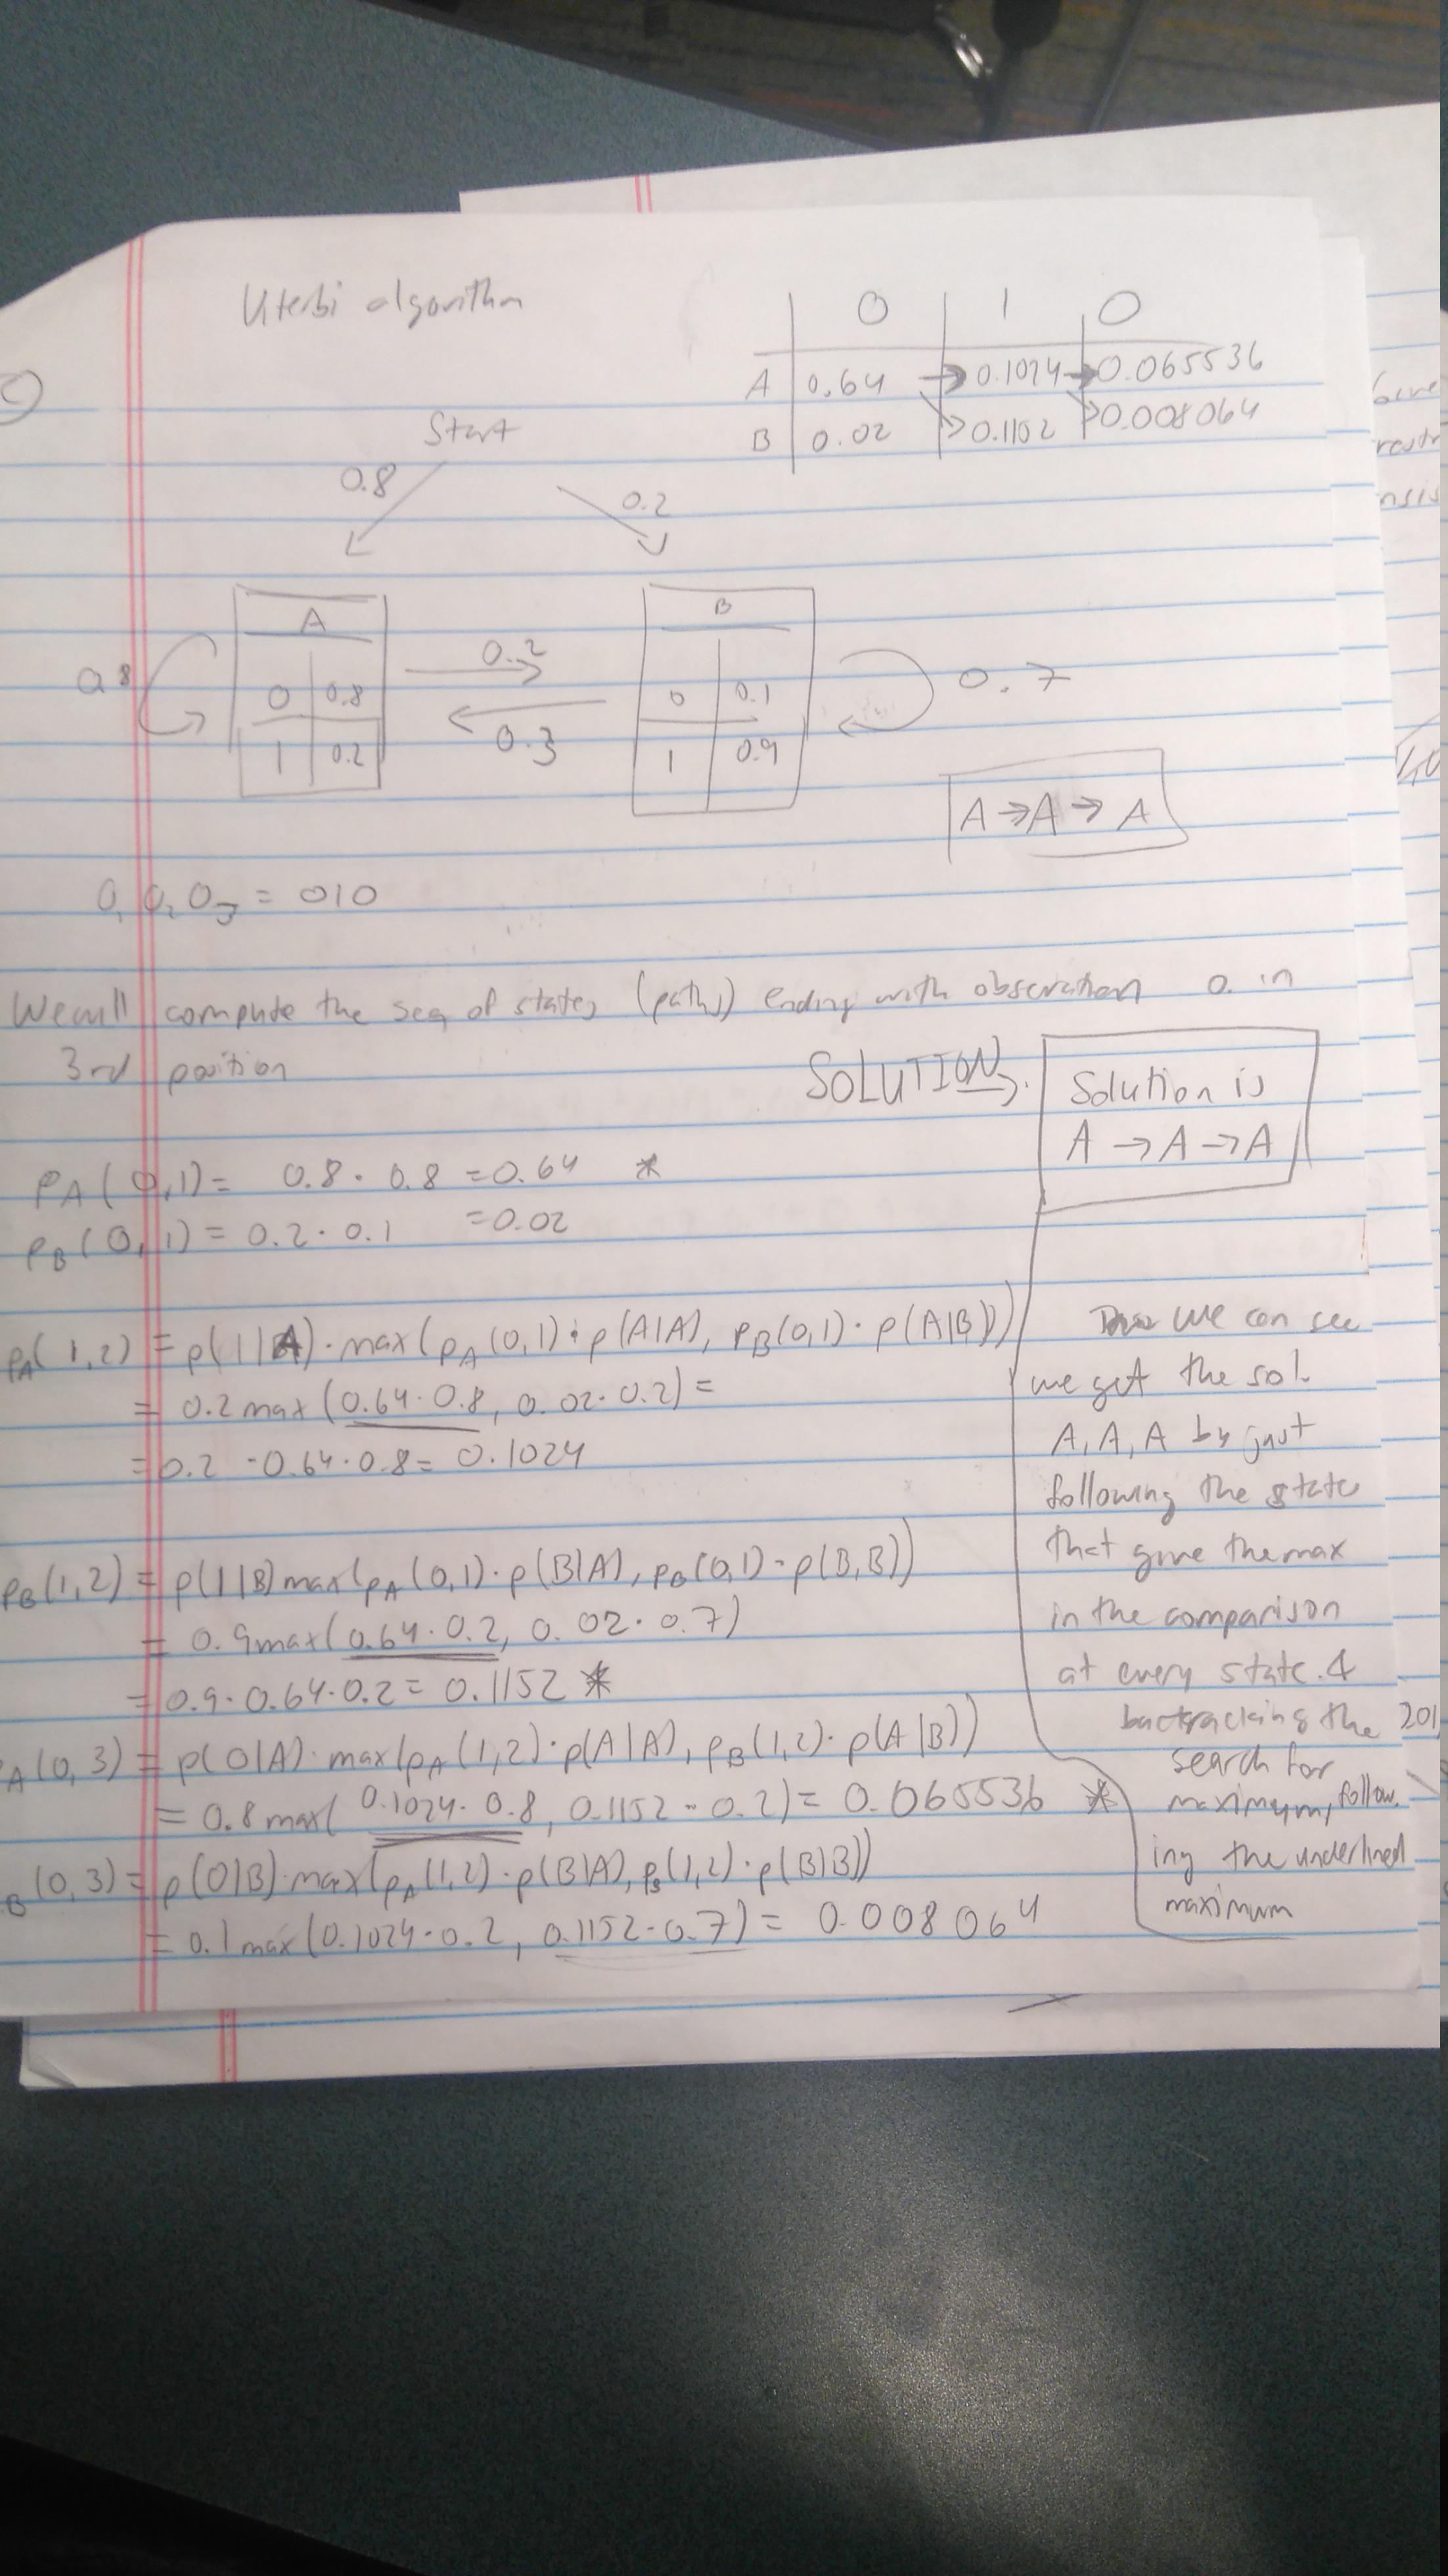
\includegraphics[width = 13cm]{hw6_1c.jpg}
\caption{\textbf{Problem 1 part c:} Image showing the work for 1 sequence 010}
\end{figure}

\end{proof}

\newpage
\begin{problem}
\normalfont 
Problem 2
\end{problem}

\begin{proof}



\end{proof}

\newpage
\begin{problem}
\normalfont 
Problem 3
\end{problem}

\begin{proof}

\begin{figure}[!htbp]
\centering
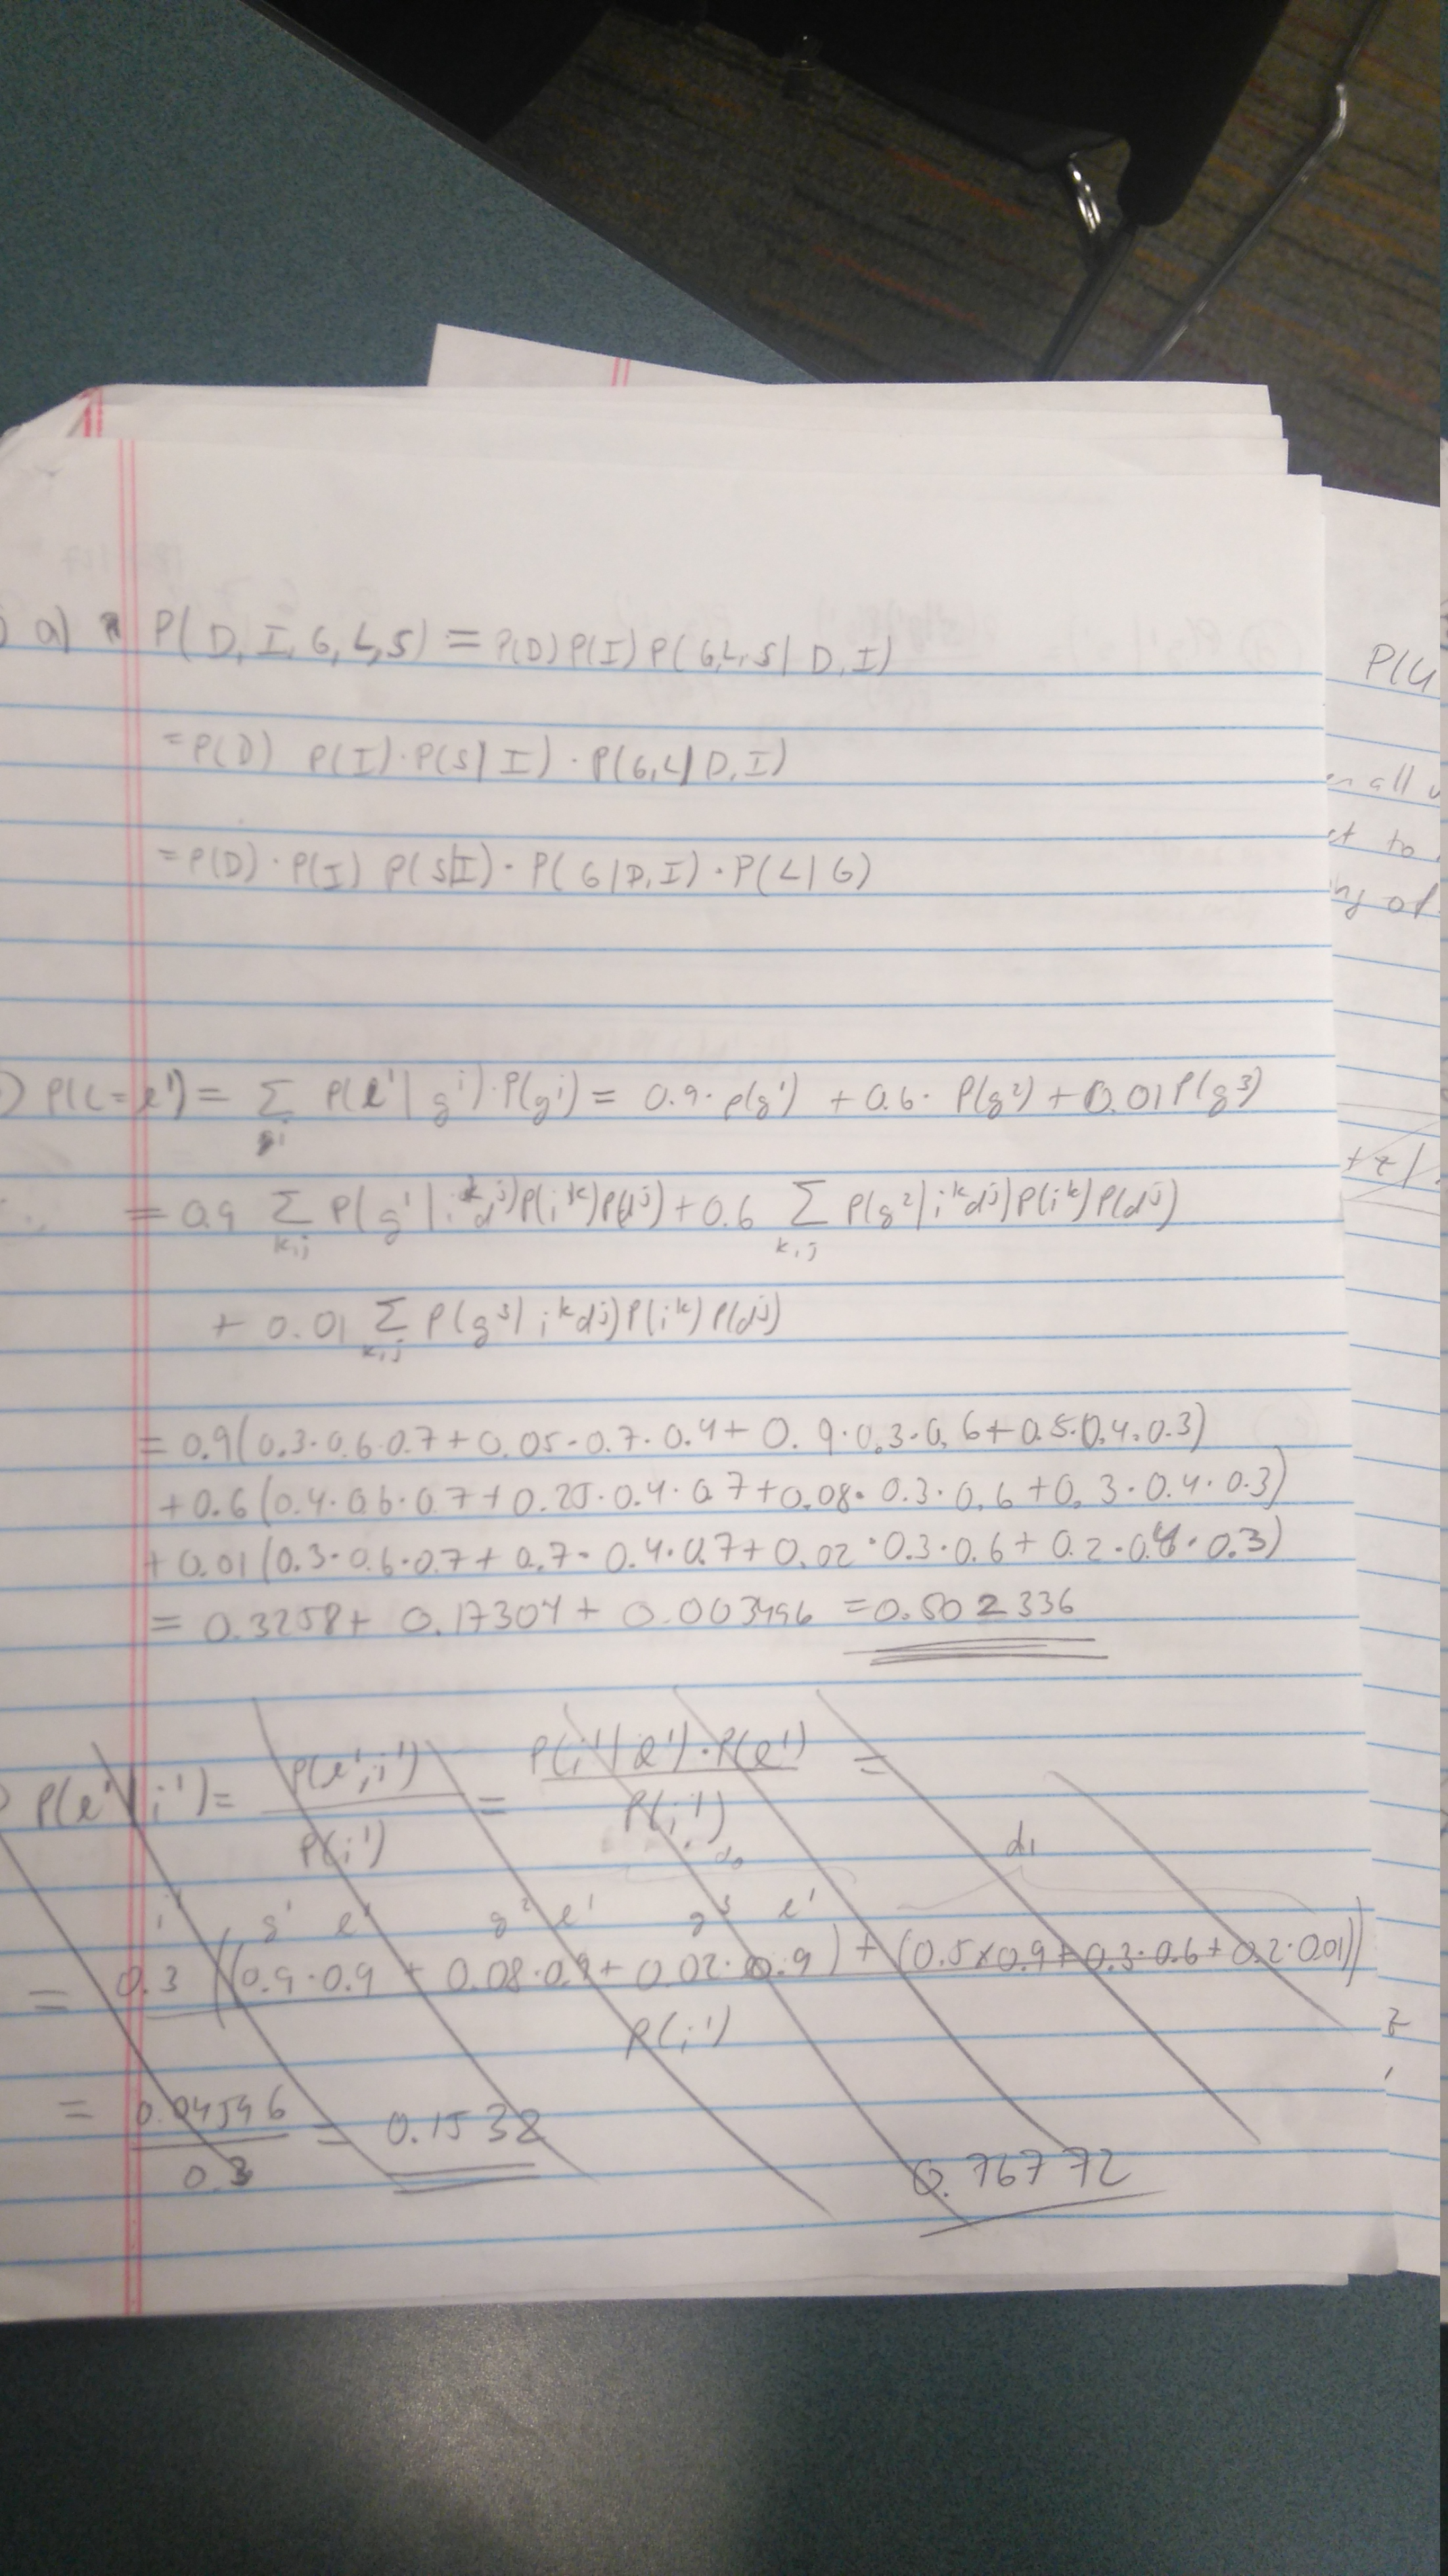
\includegraphics[width = 13cm]{hw6_3ab.jpg}
\caption{\textbf{Problem 3} Image showing the work for problem 3 part a and b}
\end{figure}

\newpage

\begin{figure}[!htbp]
\centering
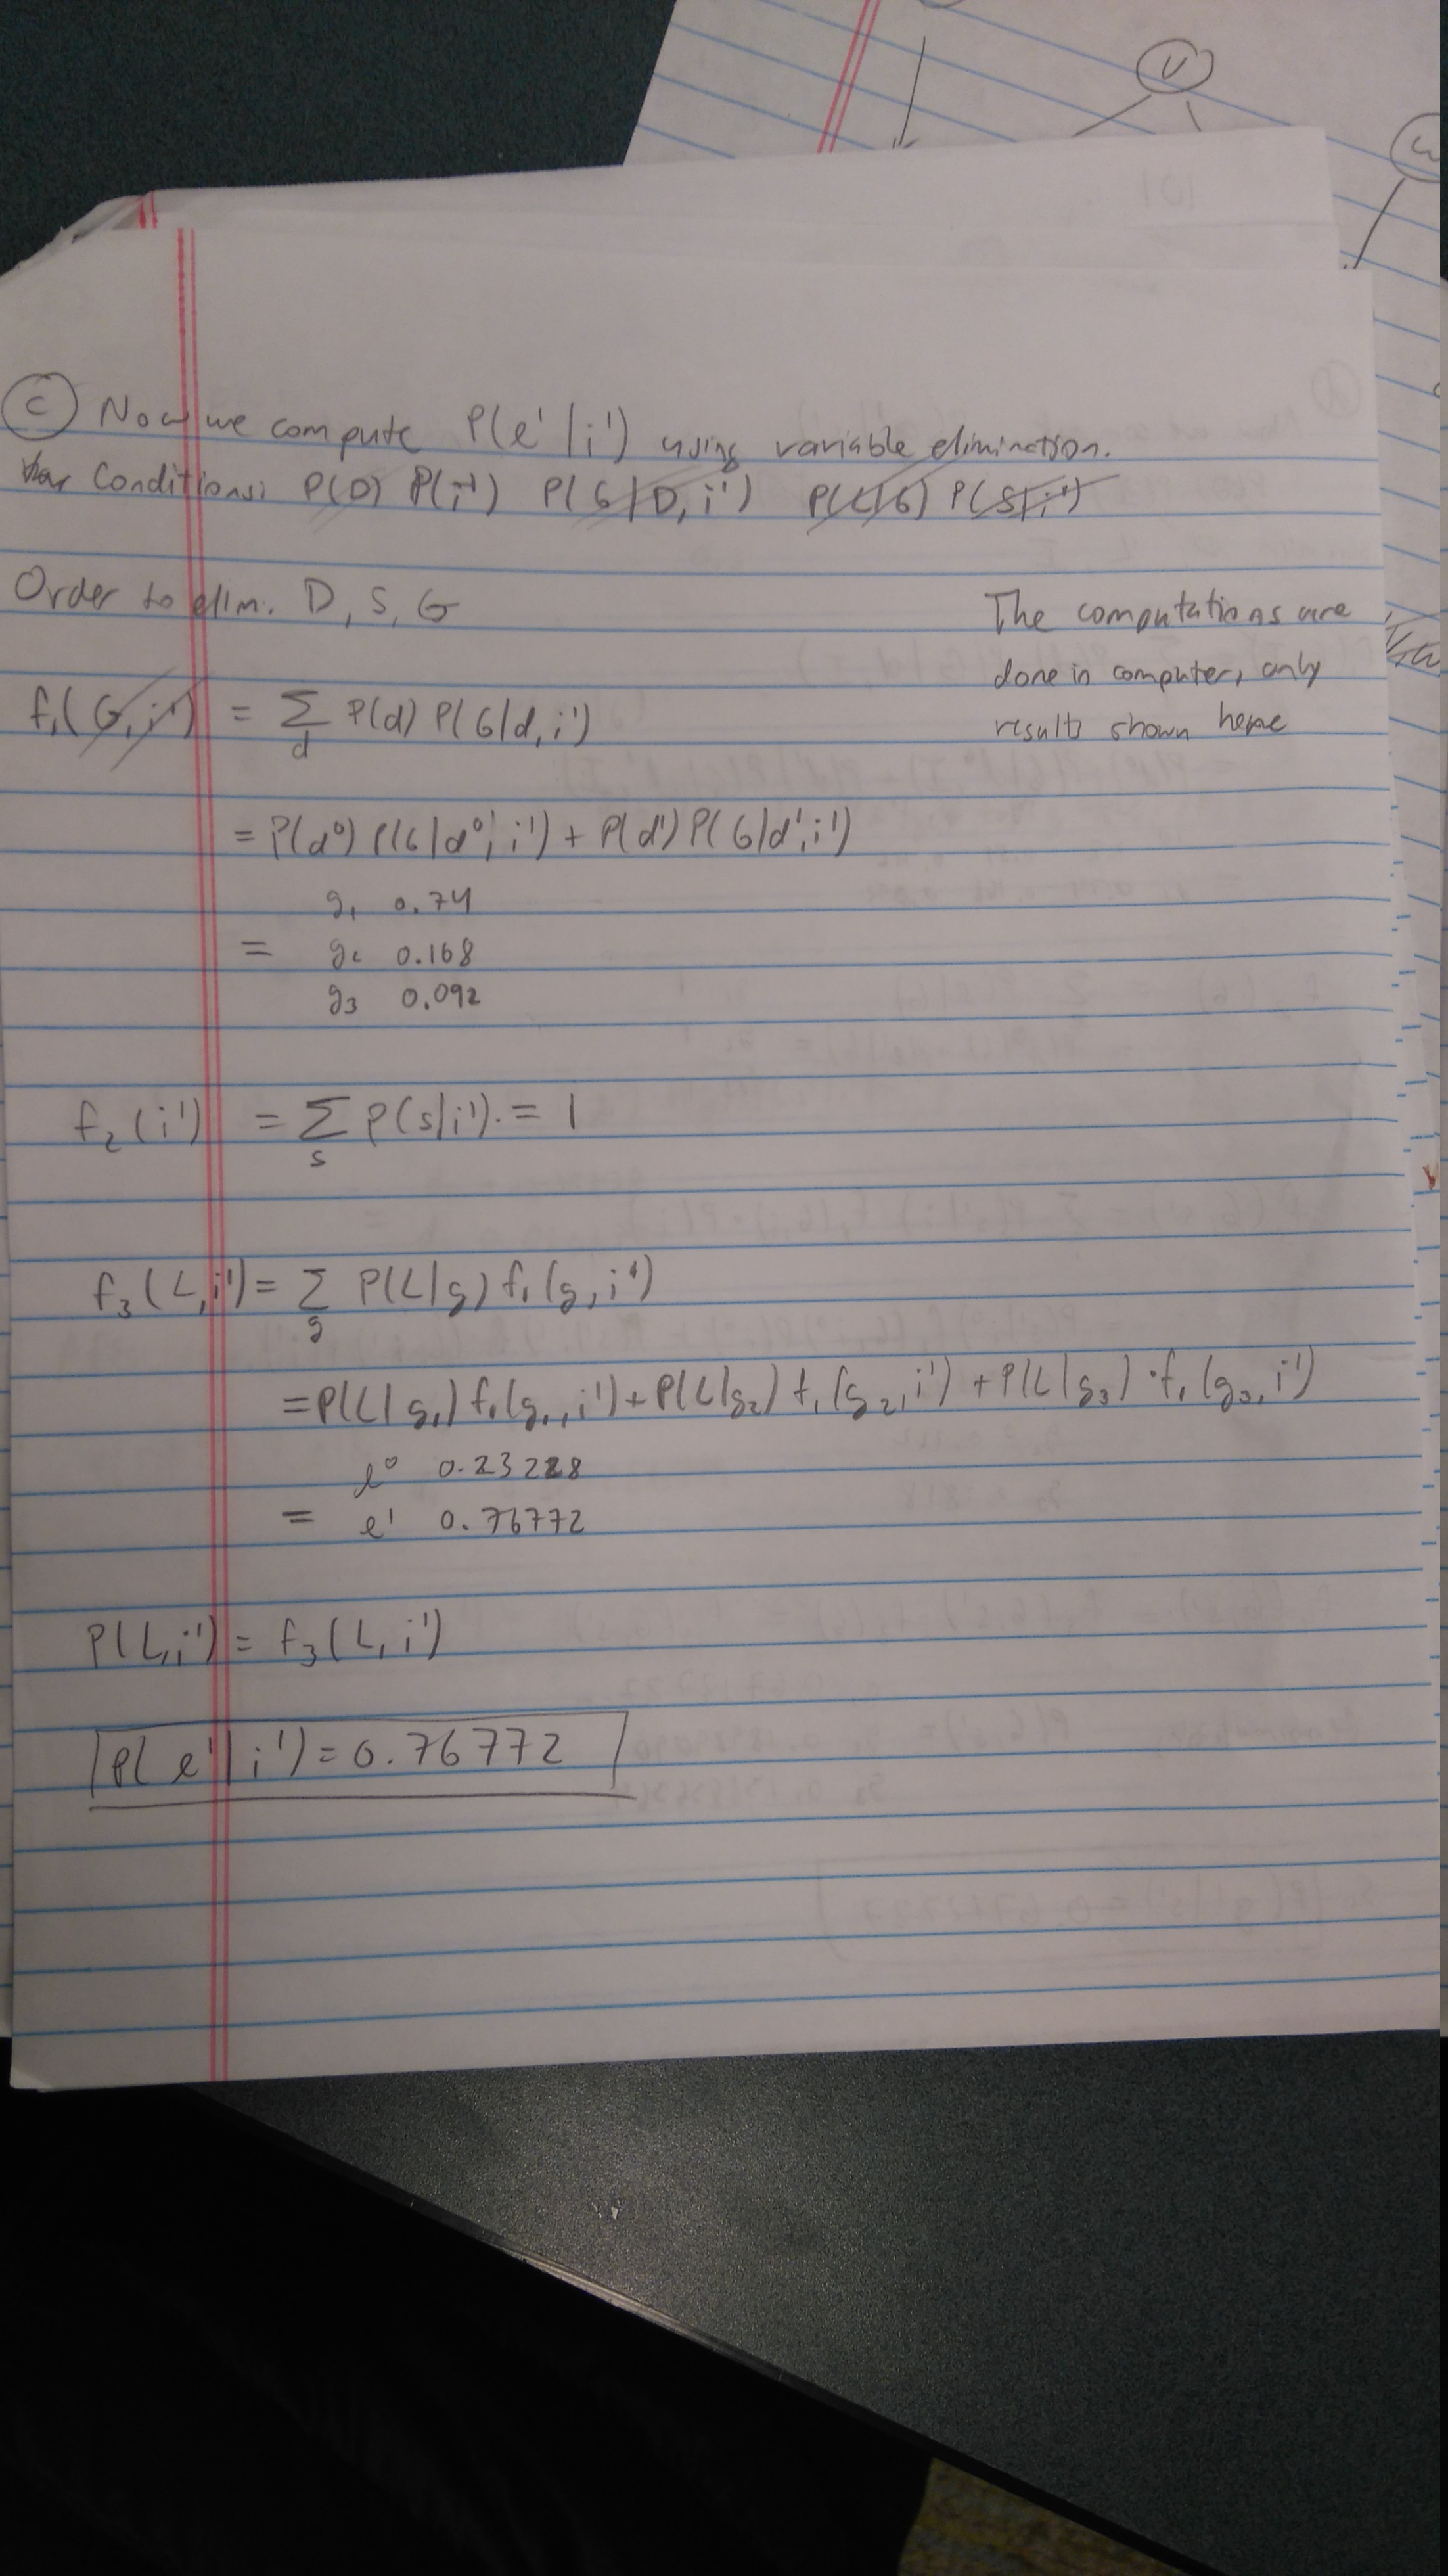
\includegraphics[width = 13cm]{hw6_3c.jpg}
\caption{\textbf{Problem 3} Image showing the work for problem 3c}
\end{figure}


\newpage

\begin{figure}[!htbp]
\centering
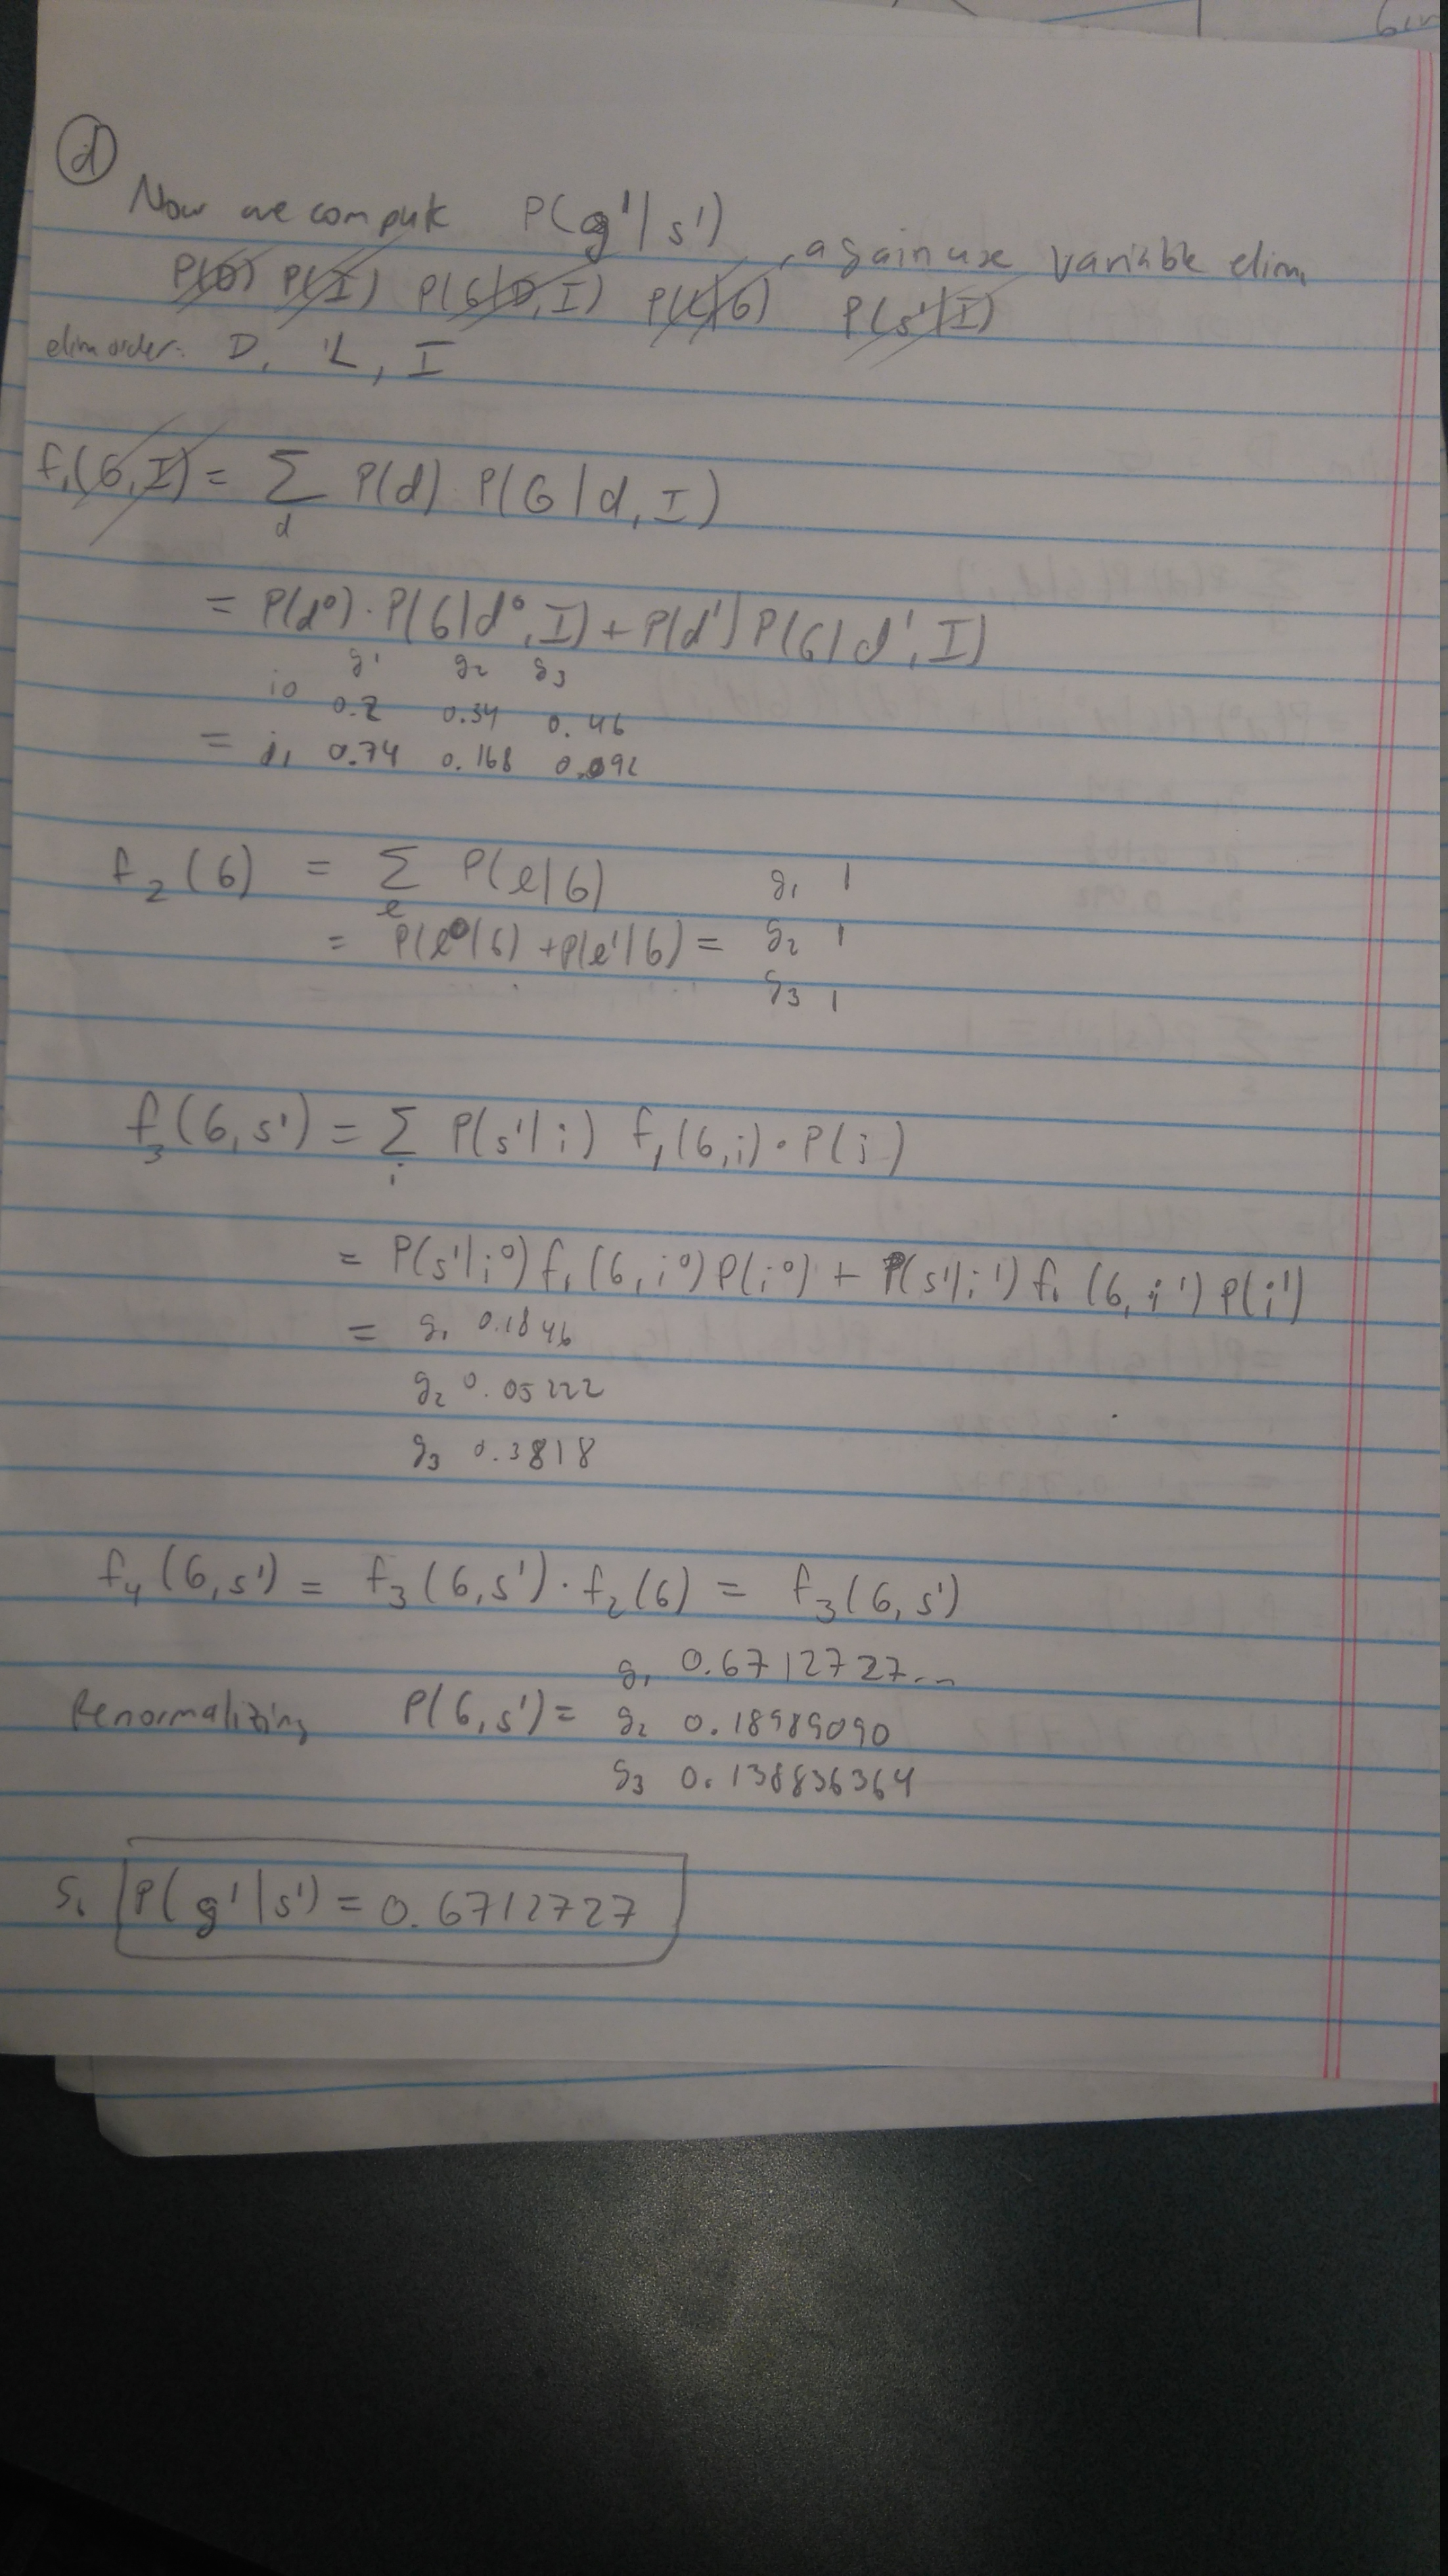
\includegraphics[width = 13cm]{hw6_3d.jpg}
\caption{\textbf{Problem 3} Image showing the work for problem 3d}
\end{figure}

\newpage

\begin{figure}[!htbp]
\centering
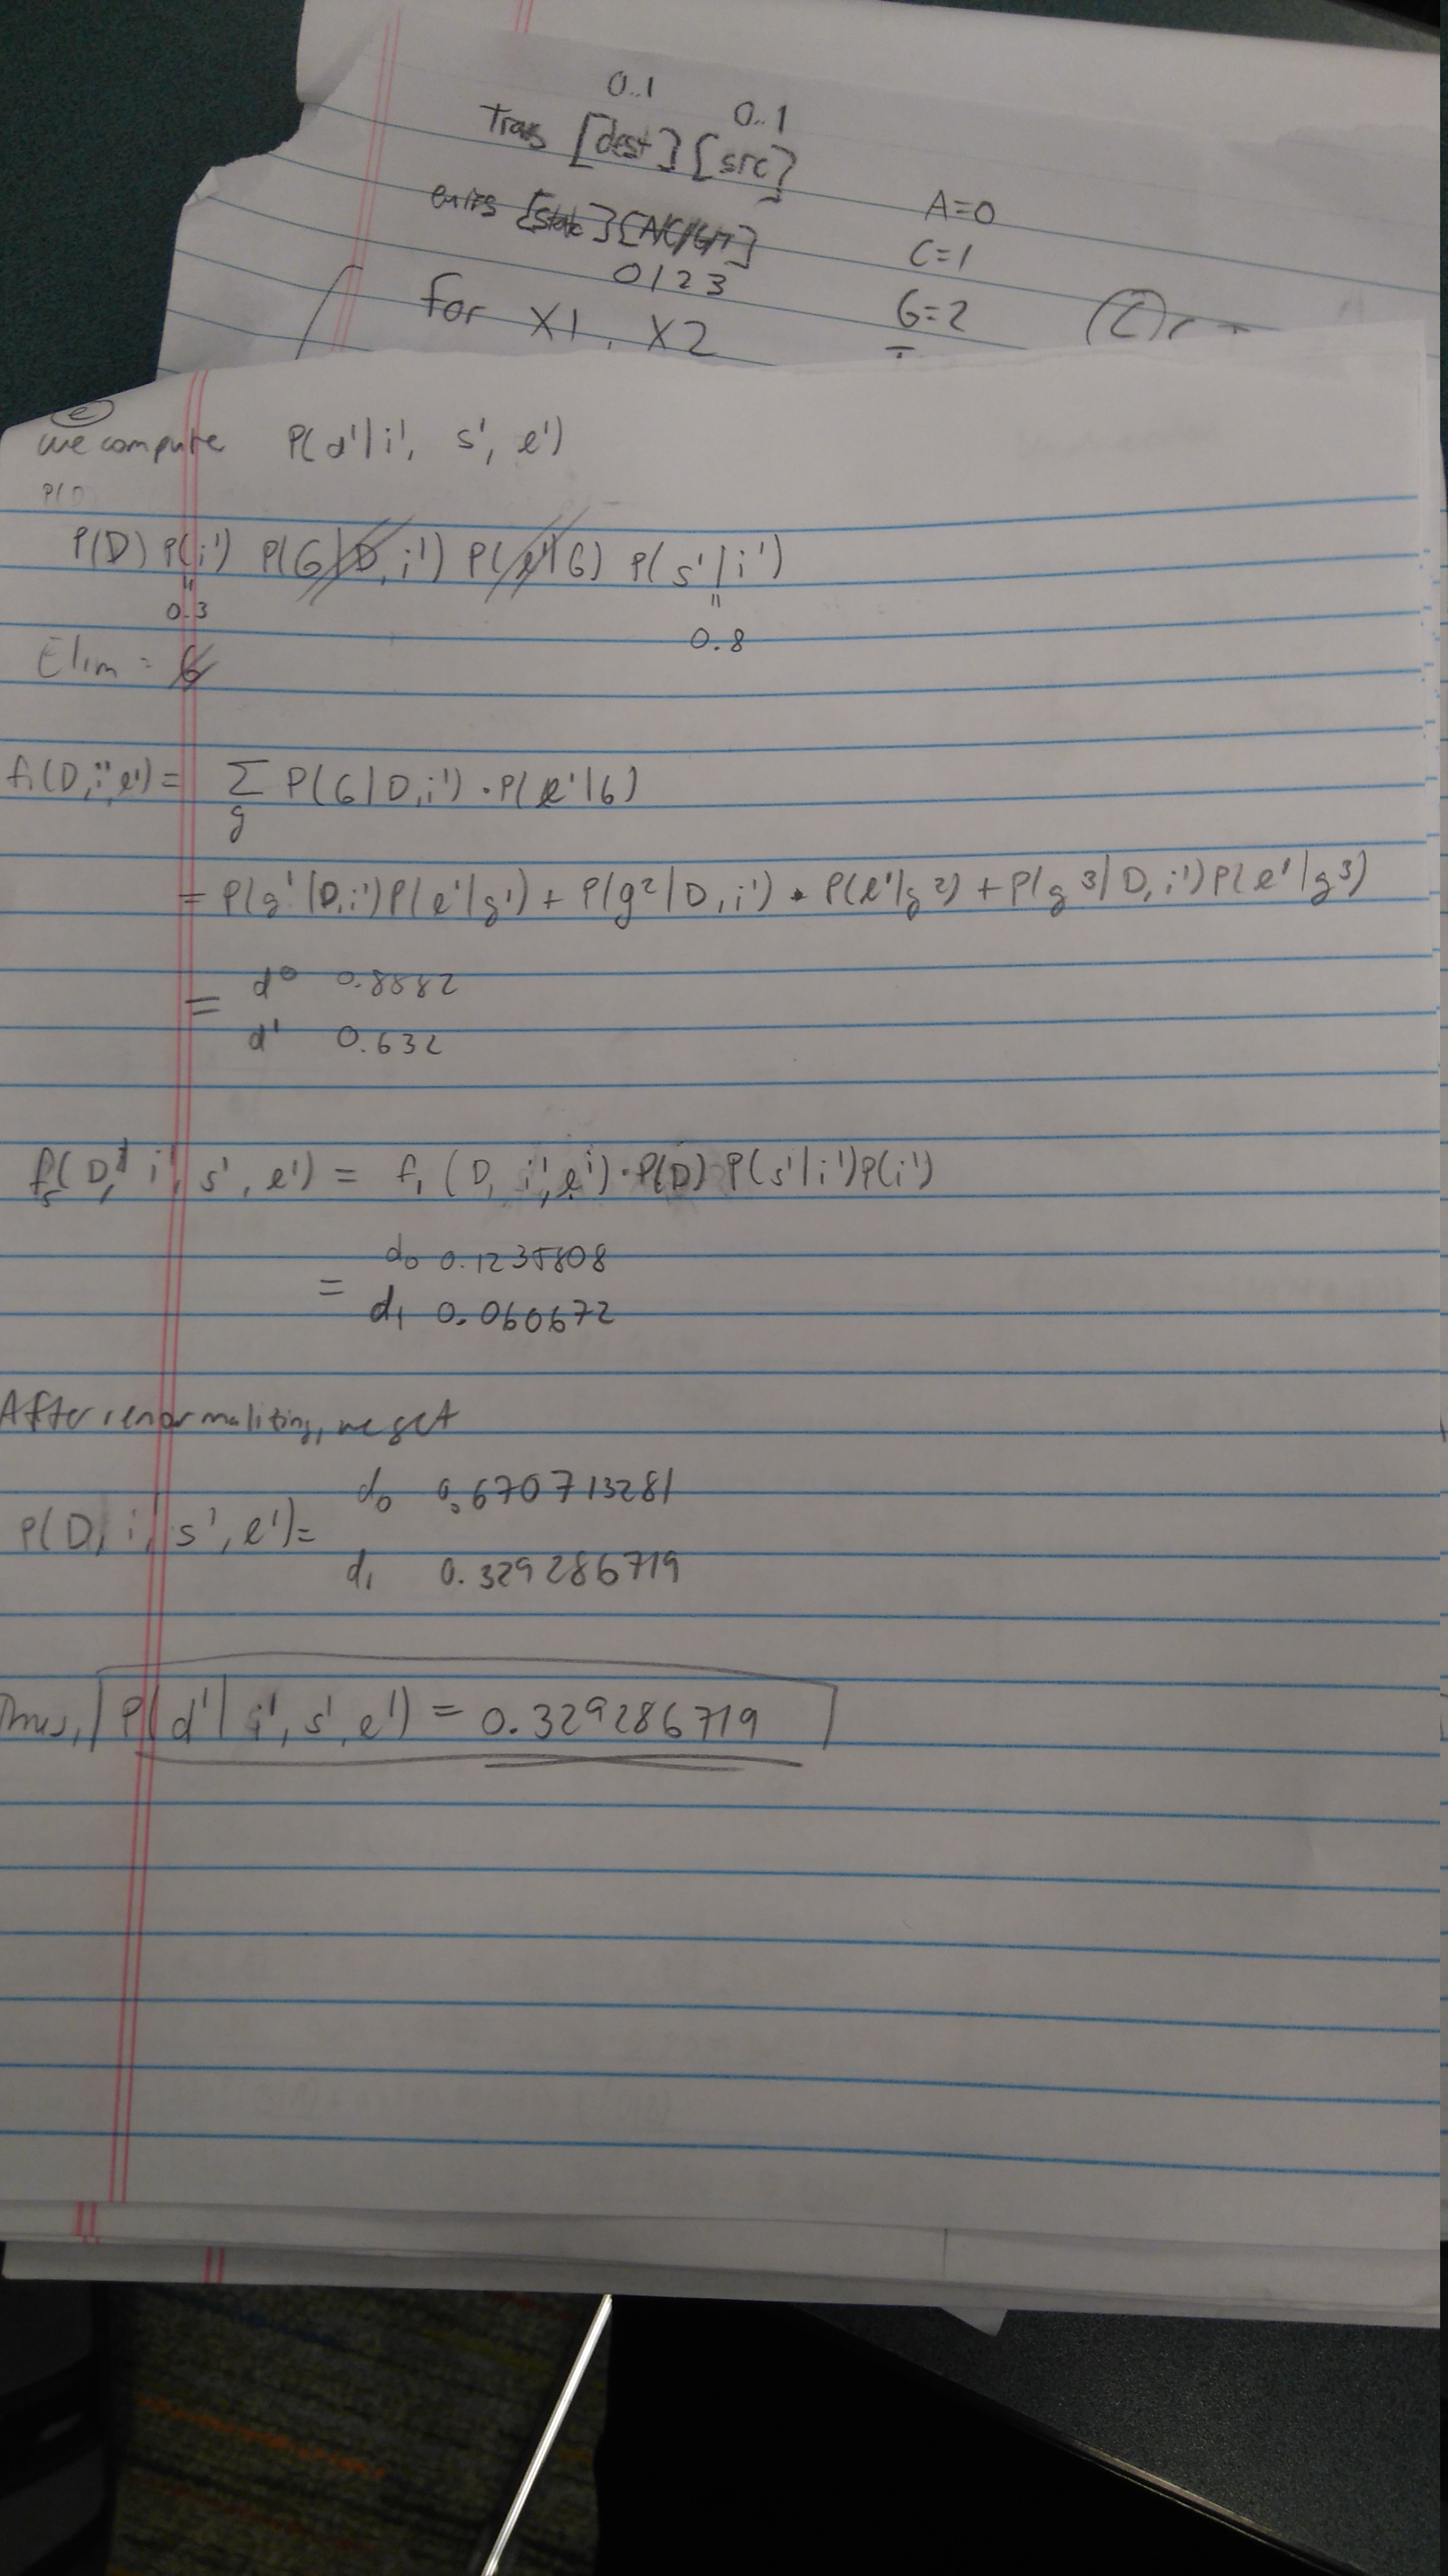
\includegraphics[width = 13cm]{hw6_3e.jpg}
\caption{\textbf{Problem 3} Image showing the work for problem 3e}
\end{figure}

\end{proof}


\newpage

\begin{problem}
\normalfont 
Problem 4
\end{problem}

\begin{proof}

The two principal directions are:

vector 1 $= \left\{ \left[ \begin{matrix} -0.24959319 \\ 0.31318631 \\ -0.24705298 \\ -0.06642483 \\ 0.07998801 \\ 0.24796042 \\ -0.77360385 \\ -0.14534989 \\ -0.04552843 \\ -0.25537919 \\ 0.0881295 \\ 0.10648068 \\ -0.01737437 \end{matrix}\right] \right\}$

and vector 2 $ = \left\{ \left[ \begin{matrix}  0.25652131 \\ 0.32130825\\ -0.29855754 \\-0.12862481 \\ 0.32209839 \\  0.31167125\\ 0.28754911 \\ 0.39962744 \\ 0.08089873 \\-0.36040796\\ -0.07174148\\ -0.26369745] \end{matrix}\right] \right\}$


Also, the scatter plot of this first two principal components is:

\begin{figure}[!htbp]
\centering
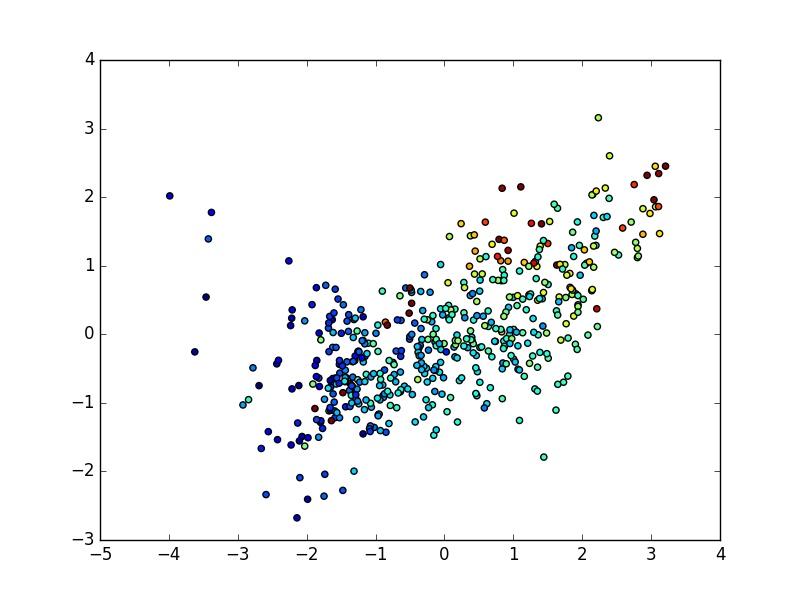
\includegraphics[width = 13cm]{PCA_2.jpg}
\caption{\textbf{Problem 4} Image showing scatter plot with color}
\end{figure}

\end{proof}

\end{document}